%!TEX root = ../dissertation.tex
\chapter{Leveraging ecological rationality to learn how to learn}
\label{chap:causal}

The study of the role of the environment in the kinds of inference strategies intelligent systems learn opens up the possibility of leveraging this insight to build artificial systems with desirable learning properties. In the previous Chapter we saw how standard machine-learning approaches -- which are based on optimization of a cost function in expectation over several training examples -- are susceptible to structure in the space of queries, and can learn ecologically rational heuristics. We also saw that augmentations to the environment that alter the ecological validity of the original heuristics leads to more generalizable solutions. This motivates a new direction of research. Traditional approaches to building artificial intelligence focus on engineering new models and architectures that can make more efficient use of computational resources to learn complex concepts and behaviors, on fairly standardized datasets. By considering the role of the environment in shaping inference, we open up a new set of ways to engineer artificially intelligent systems by directly manipulating their training environment.

Meta-learning, or `learning to learn'\cite{schmidhuber1987evolutionary, thrun2012learning} is an approach in machine-learning where rather than learning to perform a single task, systems encounter series of related tasks. Over this experience they learn commonalities across these related tasks that allow them not only to become better at solving each task at hand, but also to solve previously unobserved tasks from the same distribution, with little new experience. This dramatically reduces the sample complexity of machine-learned algorithms, enabling them to perform so-called `few-shot' learning\citep{vinyals2016matching, ravi2016optimization}.

I will focus on a different aspect of meta-learning. In this chapter, I show how one can combine the framework of learning the learning or inference procedure itself from data, with the insight that the training environment largely controls the representations acquired, to elicit complex behaviors from very simple models simply by engineering its training distribution. In particular, I will demonstrate how a simple neural network architecture, trained with trial and error learning from reinforcement, can exhibit causal reasoning and active information seeking behaviors. The absence of causal sensibilities in artificial intelligence has been a long standing criticism of the current approaches to it like machine learning. \citep{pearl88probabilistic, pearl2000} I show that agents trained this way can learn strategies that effectively probe, uncover, and leverage the specific kinds of causal structure in their environment to perform causal reasoning in related, held-out tasks in order to obtain rewards, select informative interventions, draw causal inferences from observational data, and make counterfactual predictions. This work also lays the groundwork for causally directed, structured exploration in artificial intelligence using agents that can perform and causally interpret experiments in their environments to generate their own data, much the way human children do\citep{gureckis2012self}.

I will also discuss how this direction can also offer new insights into human cognition. Discovering and exploiting the causal structure in the environment is a crucial challenge for intelligent agents and is present in human children, rats, and even some birds \citep{leslie1982perception,gopnik2001causal,gopnik2004theory,blaisdell2006causal, lagnado2013causal}. However, there is much debate about the origins and form of such causal reasoning in natural intelligence\citep{waldmann2013causal, cartwright2004causation}. The emergence of causal reasoning and intervention strategies from simpler reinforcement learning algorithms using a meta-learning framework provides a possible model for how causal reasoning emerges. Empirical findings in human behavioral research also suggest the use of context-dependent heuristic strategies in how adults implement causal inference. A meta-learning model of causal inference could explain some of these findings via similar mechanisms as those studied previously in this thesis for the emergence of ecologically rational heuristic strategies in humans and machines (Chapters \ref{chap:LTI} and \ref{chap:sentences}).

\section{Meta-learning causal reasoning}

Real-world situations often require us to reason about cause and effect. Although causal reasoning has commonly been touted as an essential component of natural intelligence, characterizing these abilities in humans and understanding how they emerge and develop through childhood are still active areas of research in cognitive science and psychology \citep{waldmann2013causal, cartwright2004causation}. 

Empirical work in human developmental research suggests that causal knowledge, and the ability to acquire and exploit it, might not necessarily reflect the operation of some general and innate algorithm, but instead emerges through learning\citep{saxe2006perception, meltzoff2007infants, bonawitz2010just, carey2009origin}.\footnote{While studies suggesting innate causal understanding exist\citep{liu2019origins, schulz2007preschool}, it is nonetheless a valuable direction to better understand how a notion of causality and causal inference might be learned.} Evidence from studies in adult causal reasoning also show that their causal theory is not entirely normative, and is instead graded and often tends towards associative reasoning \citep{rehder2014independence, rehder2017failures, fernbach2010neglect, fernbach2013cognitive}. Further, these observed behavioral patterns are not consistent and show significant variation depending on mechanisms \citep{lombrozo2010causal}, and exposure \citep{krynski2007role}. The theory that causality is learned from experience offers a potential explanation for these findings -- different experiences potentially support different kinds and extents of causal reasoning, and exact normative causal inference may not universally be the best adaptation to all aspects of the world humans operate in.

This gives rise to the question of what learning mechanisms allow causal understanding to be acquired from experience. In this work, we demonstrate how causal reasoning can arise in agents trained using meta-learning
% \footnote{Meta-learning refers to a broad range of approaches in which aspects of a learning algorithm itself are learned from the data. Details and formlisms are discussed in the Supplementary Materials.} 
simply through interaction with environments that contain causal structure. In particular, we use a ``meta-reinforcement learning'' framework \citep{duan2016RL2,wang2016}. We chose reinforcement learning (RL) as the base learning paradigm since RL is based on interactions of an agent with the environment through actions. This allows for \textit{interventions} which are an essential part of causal reasoning. This methodology has also been shown to give rise to complex policies that exploit structure in the task distribution, such as negotiating the explore-exploit trade-off in bandits \citep{wang2016, wang2018}, using episodic memory \citep{ritter2018been}, and amortizing Bayesian filtering to solve sequential problems\citep{ortega2019meta}.

A key prediction of learning causality from experience, like in our framework, is that the (causal) inference algorithm learned should reflect the structure of the environment and the data received by the agent. If normative causal reasoning provides an advantage, and is possible given the observed data and the structure of the environment, then an agent should be able to learn it. However, other kinds of experiences might lead to different algorithms that vary on the spectrum of how `causally-aware' they are. In this paper, we test these predictions in 5 experiments. We see that architecturally identical agents can learn different strategies for reasoning about causal structure depending on the kinds of experiences gathered during training. 

Finally, formal approaches to causal identification (determining the causal graph from data) often require large amounts of data \citep{geiger1990identifying,spirtes2000causation,verma1991equivalence}, and inference in the constructed causal graphs is also computationally expensive \citep{jordan2002graphical}. In real-world environments, humans operate under time, data, and resource constraints, dealing with uncertainty in model structure as well as non-stationarity. Agents that learn aspects of the learning algorithm directly from experience will adapt to statistical structure in their specific environment and task, and could utilize useful abstract priors (or inductive biases) from other episodes that can be difficult to formally specify. Such adaptations amortize much of the computation over previous experience and could allow better performance than formal approaches under ecological constraints\citep{dasgupta2019theory,gershman2015computational,gigerenzer2009homo,lieder2017strategy,todd2007environments}.  

The purpose of this work is not to propose a new algorithmic solution to causal inference per se. Rather, we highlight that this is the first demonstration of causally-aware inference procedures emerging from simple reinforcement learning procedures in an unstructured model through interaction with an environment the rewards causal understanding. This demonstrates that structured training environments and ecological rationality in machine learning can be leveraged to give rise to complex behaviors. Further, we argue that our meta-learning approach has compelling links to human causal reasoning in terms of a) how a theory of causality could be learned, b) the graded notion of causality in humans, and c) resource efficiency by meta-learning inductive biases. Resource efficient causal inference based on leveraging statistical structure, is also useful for and an active area of research in machine learning \citep[e.g.][]{bengio2019meta, heckerman1995learning,magliacane2018domain,parascandolo2017learning,mitrovic2018causal}.

\section{Background}

\subsection{Related Work}

\citet{goodman2011learning} demonstrated how an abstract notion of causality in humans can be learned from experience, with hierarchical Bayesian inference. Our approach is similar to this as meta-learning can also be framed as hierarchical Bayesian inference \citep{grant2018recasting}. However, these approaches provide complementary advantages: we discuss in later sections how the meta-learning approach outlined here can be combined with more structured approaches to causal inference, to best leverage these complementary advantages. While formal theory learning (as in \citet{goodman2011learning}) is systematic and generalizes across domains, it requires the pre-specification of discrete primitives and an expensive zero order (stochastic search) optimization to learn the correct theory built from these primitives. \citep{schulz2012finding, bramley2018grounding} A restrictive choice of primitives limits the space of possible theories, while a generous choice makes the optimization very expensive. This approach also leaves open the question of the origin of these discrete primitives and how they might be plausibly implemented in the brain. Our method avoids these assumptions and instead uses a first order (gradient-based) optimization method that leverages learning signals from the environment, thus discovering emergent structure directly from experience \citep{mcclelland2010letting}. This also provides a basis for modeling the domain/function specificity \citep{krynski2007role, lombrozo2010causal} seen in humans. Since our model is implemented with a deep neural network, which can be universal approximators \citep{siegelmann1995computational, hornik1991approximation}, it can implement different graded causal theories that don't conform to purely normative accounts, in a neurally-plausible distributed representation.  This could give rise to graded causal reasoning behaviors analogous to those seen in humans \citep{rehder2014independence, rehder2017failures, fernbach2010neglect, fernbach2013cognitive}. 


% The only key assumption in our framework is the existence of a reinforcement learning mechanism, which is plausibly inbuilt via evolution -- evidence for basic RL mechanisms are present as far back as invertebrates \citep{niv2002evolution, brembs2002operant, walters1981associative}. , using robust, neurally plausible, distributed representations. 
% Further, the reasoning framework in our work is parameterized by a deep neural network, which can be universal approximators \citep{siegelmann1995computational, hornik1991approximation}, and thus can naturally capture different graded forms of reasoning that don't conform to purely normative accounts. 
% Second,  . Third, the theory that is learned will leverage the specific structure present in the data and thereby adapts to different environments and contexts. This provides a basis for modelling the kinds of . Finally, our method uses first order (gradient-based) optimization that utilizes learning signals to ``move in the right direction'' and avoids the expensive zero order (stochastic search) optimization that learning with formal discrete theories usually requires. This makes the learning process in our model more efficient, as well as more reusable (\textit{amortizable}) across queries.

Bengio et al \citep{bengio2019meta} propose a meta-learning approach to utilize explicit, pre-specified statistical properties of interventions to isolate and disentangle causal variables in a supervised learning setting. Our work shows how a spectrum of `causally-aware algorithms' can arise from utilizing several different kinds of implicit, unspecified statistical structure in the environment. Our reinforcement learning approach further allows the agent to directly interact with the environment to also simultaneously learn an experimental policy that utilizes this underlying structure. Denil et al \citep{denil2016learning} showed that deep reinforcement learning agents can learn to perform actions to gain knowledge about latent, physical properties of objects, but do not explore explicit causal inference.

\subsection{A brief introduction to causal reasoning}

%By combining graph theory and probability theory, the causal Bayesian network framework provides us with a graphical tool to formalize and test different levels of causal reasoning.\citep{pearl88probabilistic, bishop06pattern, kollerl09probabilistic, barber12bayesian, murphy12machine}. Here, we introduce a simple example of the key concepts in causal reasoning with an intuitive example, see Appendix \ref{app:causal_cbn} for further details.

Causal relationships among random variables can be expressed using \emph{causal Bayesian networks} (\CBNs~${\cal G}$)  \citep{pearl2000,spirtes2000causation,dawid07fundamentals}. Each node $X_i$ corresponds to a random variable, and the joint distribution $p(X_1, \ldots, X_N)$ is given by the product of conditional distributions of each node $X_i$ given its parent nodes $\textrm{pa}(X_i)$, i.e.~$p(X_{1:N})=\prod_{i=1}^Np(X_i|\textrm{pa}(X_i))$. 

The edges of ${\cal G}$ encode causal semantics: a directed path from $X_c$ (cause) to $X_e$ (effect) is called a causal path. The causal effect of $X_c$ on $X_e$ is the conditional distribution of $X_c$ given $X_e$ restricted to only causal paths. This restriction is an essential caveat, since the simple conditional distribution \(p(X_e|X_c)\) encodes only correlations (i.e. associative reasoning). Intervening on a node $X_c$ corresponds to removing its connection to its parent nodes  $\textrm{pa}(X_c)$, and fixing it to some value $C$ yielding a new \CBN~${\cal G}_{\rightarrow X_c = C}$. The causal effect of $X_c$ on $X_e$ is given by the conditional distribution in this new \CBN. This distribution is denoted $p_{\rightarrow X_c = C}(X_e|X_c = C)$
\footnote{In the causality literature, this distribution would most often be indicated with $p(X_e|\textrm{do}(X_c = C))$. We prefer to use $p_{\rightarrow X_c = C}(X_e|X_c = C)$ to highlight that intervening on $X_c$ results in changing the original distribution $p$ by structurally altering the \CBN.}. 

An example of \CBN~${\cal G}$ is given in Figure \ref{fig:CBN}a, where $E$ represents hours of exercise in a week, $H$ cardiac health, and $A$ age. 
Random variables are denoted by capital letters (e.g., $E$) and their values by small letters (e.g., $e$). The causal effect of $E$ on $H$ is the conditional distribution restricted to the path $E\rightarrow H$, i.e.~excluding the path $E\leftarrow A \rightarrow H$. The variable $A$ is called a \emph{confounder}, as it confounds the causal effect with non-causal statistical influence. 

Simply observing cardiac health conditioning on exercise level from $p(H|E)$ (associative reasoning) cannot answer if change in exercise levels cause changes in cardiac health (cause-effect reasoning), since there is always the possibility that correlation between the two is because of the common confounder of age. 

\begin{figure}[t!]
\centering
\subfloat[]{
\scalebox{0.85}{
\begin{tikzpicture}[dgraph]
\node at (1,0.6) {${\cal G}$}; 
\node[ocont] (A) at (1,1.5) {$A$};
\node[ocont] (E) at (0,0) {$E$};
\node[ocont] (H) at (2,0) {$H$};
\node[] at (1,2.1) {$p(A)$};
\node[] at (0,-0.7) {$p(E|A)$};
\node[] at (2,-0.7) {$p(H|A,E)$};
\draw[line width=1.15pt](A)--(E);\draw[line width=1.15pt](A)--(H);\draw[line width=1.15pt](E)--(H);
\end{tikzpicture}}}
\hskip0.3cm
\subfloat[]{
\scalebox{0.8}{
\begin{tikzpicture}[dgraph]
\node at (0.9,0.6) {${\cal G}_{\rightarrow E=e}$}; 
\node[ocont] (A) at (1,1.5) {$A$};
\node[contdec] (E) at (0,0) {$E$};
\node[ocont] (H) at (2,0) {$H$};
\node[] at (1,2.1) {$p(A)$};
\node[] at (0,-0.7) {$\delta(E-e)$};
\node[] at (2,-0.7) {$p(H|A,E)$};
\draw[line width=1.15pt](A)--(H);\draw[line width=1.15pt](E)--(H);
\end{tikzpicture}}}
% %\vspace{-0.2cm}
\caption{(a): A \CBN~${\cal G}$ with a confounder for the effect of exercise ($E$) on heath ($H$) given by age ($A$). 
(b): Intervened \CBN~${\cal G}_{\rightarrow E=e}$.}
% (see main text for details).}
% \caption{(a): A \CBN~${\cal G}$ with a confounder for the effect of exercise ($E$) on heath ($H$) given by age ($A$). (b): Intervened \CBN~${\cal G}_{\rightarrow E=e}$ resulting from modifying ${\cal G}$ by replacing $p(E|A)$ with a delta distribution $\delta(E-e)$ and leaving the remaining conditional distributions $p(H|E,A)$ and $p(A)$ unaltered.}
\label{fig:CBN}
%\vspace{-0.5cm}
\end{figure}

The causal effect of $E=e$ can be seen as the conditional distribution $p_{\rightarrow E=e}(H|E=e)$\footnote{In the causality literature, this distribution would most often be indicated with $p(H|\textrm{do}(E=e))$. We prefer to use $p_{\rightarrow E=e}(H|E=e)$ to highlight that intervening on $E$ results in changing the original distribution $p$, by structurally altering the \CBN.} on the \emph{intervened} \CBN~${\cal G}_{\rightarrow E=e}$ resulting from replacing $p(E|A)$ with a delta distribution $\delta(E-e)$ (thereby removing the link from $A$ to $E$) and leaving the remaining conditional distributions $p(H|E,A)$ and $p(A)$ unaltered (Figure \ref{fig:CBN}b).
The rules of do-calculus \citep{pearl2000,pearl16causal} tell us how to compute $p_{\rightarrow E=e}(H|E=e)$ using observations from ${\cal G}$. In this case $p_{\rightarrow E=e}(H|E=e) = \sum_A p(H|E=e,A)p(A)$\footnote{Notice that conditioning on $E = e$ would instead give $p(H|E=e)=\sum_{A}p(H|E=e,A)p(A|E=e)$.}.
Therefore, do-calculus enables us to reason in the intervened graph ${\cal G}_{\rightarrow E=e}$ even if our observations are from ${\cal G}$. This is the kind of causal reasoning possible in our observational data setting.

Such inferences are always possible if the confounders are observed, but in the presence of unobserved confounders, for many \CBN~structures the only way to compute causal effects is by collecting observations directly from the intervened graph, e.g. from ${\cal G}_{\rightarrow E=e}$ by fixing the value of the variable $E=e$ and observing the remaining variables---we call this process performing an actual intervention in the environment. In our interventional data setting the agent has access to such interventions. 

\paragraph{Counterfactual reasoning}

Cause-effect reasoning can be used to correctly answer predictive questions of the type "Does exercising improve cardiac health?" by accounting for causal structure and confounding. However, it cannot answer retrospective questions about what \textit{would have} happened. For example, given an individual $i$ who has died of a heart attack, this method would not be able to answer questions of the type "What would the cardiac health of this individual have been had she done more exercise?". This type of question requires
reasoning about a counterfactual world (that did not happen). To do this, we can first use the observations from the factual world and knowledge about the \CBN~to get an estimate of the specific latent randomness in the makeup of individual $i$ (for example information about this specific patient's blood pressure and other variables as inferred by her having had a heart attack). Then, we can use this estimate to compute cardiac health under intervention on exercise. This procedure is called the \textit{Abduction-Action-Prediction Method} \cite{pearl16causal} and is described below.

Assume, for example, the following model for ${\cal G}$ in Figure \ref{fig:CBN}: $E=w_{AE}A + \eta$, $H=w_{AH}A+w_{EH}E+\epsilon$,
where the weights $w_{ij}$ represent the known causal effects in $\cal G$ and $\epsilon$ and $\eta$ are terms of (e.g.) Gaussian noise that represent the latent randomness in the makeup of each individual. These noise variables are zero in expectation, so without access to their value for an individual we simply use ${\cal G}$: $E=w_{AE}A$, $H=w_{AH}A+w_{EH}E$ to make causal predictions. Suppose that for individual $i$ we observe: $A = a^i$, $E = e^i$, $H = h^i$. We can answer the counterfactual question of "What if individual $i$ had done more exercise, i.e.~$E=e'$, instead?" by: a) \emph{Abduction:} estimate the individual's specific makeup with $\epsilon^i=h^i-w_{AH}a^i-w_{EH}e^i$, b) \emph{Action:} set $E$ to more exercise $e'$, c) \emph{Prediction:} predict a new value for cardiac health as $h'=w_{AH}a^i+w_{EH}e'+\epsilon^i$. 

\subsection{Memory-based Meta-learning}
\label{sec:meta-formalism}

Meta-learning refers to a broad range of approaches in which aspects of the learning algorithm itself are learned from the data. Many individual components of deep learning algorithms have been successfully meta-learned, including the optimizer \citep{andrychowicz2016learning}, initial weight parameters, \citep{finn2017model}, a metric space \citep{vinyals2016matching}, and use of external memory \citep{santoro2016meta}. 

Following the approach of \citep{duan2016RL2,wang2016}, the entire inner loop of learning is implemented by a recurrent neural network (RNN), and we train the weights of the RNN with model-free reinforcement learning (RL). The RNN is trained on a broad distribution of problems which each require learning. Consider a distribution ${\cal D}$ over Markov Decision Processes (MDPs). We train an agent with memory (in our case an RNN-based agent) on this distribution. In each episode, we sample a task $m\sim {\cal D}$. At each step $t$ within an episode, the agent sees an observation $o_t$, executes an action $a_t$, and receives a reward $r_t$. Both $a_{t-1}$ and $r_{t-1}$ are given as additional inputs to the network. Thus, via the recurrence of the network, each action is a function of the entire trajectory ${\cal H}_{t}=\{ o_0, a_0, r_0, \dots, o_{t-1}, a_{t-1}, r_{t-1}, o_t\}$ of the episode. Because this function is implemented by the neural network, its complexity is limited only by the size of the network. When trained in this way, the RNN is able to implement a learning algorithm capable of efficiently solving novel learning problems in or near the training distribution.

Learning the weights of the RNN by model-free RL can be thought of as the "outer loop" of learning. The outer loop shapes the weights of the RNN into an "inner loop" learning algorithm, which plays out in the activation dynamics of the RNN and can continue learning even when the weights of the network are frozen. The inner loop algorithm can also have very different properties from the outer loop algorithm used to train it. For example, this approach has been used to negotiate the exploration-exploitation tradeoff in multi-armed bandits \citep{duan2016RL2, wang2016}, learn algorithms which dynamically adjust their own learning rates \citep{wang2016,wang2018}, and perform one-shot learning using external memory \citep{santoro2016meta}. In the present work we explore the possibility of obtaining a causally-aware inner-loop learning algorithm.

\section{Experimental setup}
\label{sec:probspec}
Our goal is to demonstrate that causal reasoning can arise from meta-reinforcement learning. Further, we demonstrate that depending on the kinds of data the agents see during training, the kind of causal reasoning learned varies. Our agents learn to leverage statistical structure in different kinds of available information, to carry out different kinds of causal reasoning. In this section, we first briefly formalize how causal inference depends on the environment,

% \begin{itemize}%[leftmargin=*]
% \setlength{\itemsep}{-2pt}  
% %\setlength{\parskip}{-4pt}
% \setlength{\partopsep}{-20pt}
% \setlength{\parsep}{-20pt}
% %%\vspace{-7pt}
% \item An observational environment~(Experiment~1), only allows the agent to obtain passive observations. Access to this type of data allows an agent to infer correlations (\emph{associative reasoning}) and, depending on the structure of the environment, some causal effects (\emph{causal reasoning}). 
% \item An interventional environment~(Experiment~2), allows the agent to act in the environment by setting the values of some variables and observing the consequences of these actions on other variables. Access to this type of data facilitates estimating causal effects.
% \item An additional level of sophistication comes from \textit{counterfactual} environments -- we provide results concerning this setting in the Supplementary Material. 
% %%\vspace{-8pt}
% \end{itemize}


Different kinds of environments support different kinds of causal reasoning. It is often possible to compute $p_{\rightarrow X_c = C}(X_e|X_c = C)$ (i.e. causal reasoning) using observations from ${\cal G}$\footnote{When the \CBN~${\cal G}$ is known, this process can be formalized as do-calculus \citep{pearl2000,pearl16causal}. In our case the \CBN~ will not be directly provided, and the agent must simultaneously perform causal identification using samples from ${\cal G}$ \citep{heckerman1995learning}.}. I investigate this kind of causal reasoning in Experiment 1 (Observational Environments). However, in the presence of unobserved confounders (an unobserved variable that affects both $X_c$ and $X_e$), this is, in general , no longer possible \citep{pearl2000}. The only way to compute causal effects $p_{\rightarrow X_c = C}(X_e|X_c = C)$ in this case is by collecting observations directly from the intervened graph ${\cal G}_{\rightarrow X_c = C}$. In Experiment 2 (Interventional Environments), I investigate this kind of causal reasoning, by allowing agent to perform interventions on the environment. An additional level of sophistication comes from \textit{counterfactual} environments, where the agent must answer a retrospective question. This requires the additional step of \textit{abduction} where the individual idiosyncrasy in the specific case at hand must be inferred and incorporated into the counterfactual prediction. I discuss these results in Experiment 3 (Counterfactual Environments).

% It is often possible to compute $p_{\rightarrow X_c = C}(X_e|X_c = C)$ (i.e. \textit{causal reasoning}) using observations from ${\cal G}$\footnote{When the \CBN~${\cal G}$ is known, this process can be formalized as do-calculus \citep{pearl2000,pearl16causal}. In our case the \CBN~ is not directly provided, and the agent must simultaneously perform causal identification using samples from ${\cal G}$ \citep{heckerman1995learning}.}. This is the kind of causal reasoning possible in our observational environment outlined above. However, in the presence of unobserved confounders (an unobserved variable that affects both $X_c$ and $X_e$), this is, in general , no longer possible \citep{pearl2000}. The only way to compute causal effects in this case is by collecting observations directly from the intervened graph ${\cal G}_{\rightarrow X_c = C}$. This kind of causal reasoning is possible in our interventional environment outlined above as the agent has access to such interventions.

\subsection{Task Setup}
\label{sec:task}

In our experiments, we use a simple framework that has some key properties relevant to ecologically realistic causal reasoning. First, the number of variables over which inference is carried out is small. Second, the amount of data available is limited. Third, agents can actively seek out information by interacting with the environment rather than only receiving passive input. This facilitates future work in drawing parallels to human causal reasoning, as well as permits a simple and clear demonstration of the effects of interest.

In each episode the agent interacts with a different \CBN~${\cal G}$ with $N$ variables. The structure of ${\cal G}$ is drawn randomly from the space of constraints described below. Each episode consists of $T$ steps, which are divided into two phases: an \emph{information phase} and a \emph{quiz phase}. The information phase corresponds to the first $T-1$ steps and allows the agent to collect information from ${\cal G}$. Note that ${\cal G}$ is never directly provided to the agent, but is only observed through $T-1$ samples. Further, the agents in the different experiments are architecturally identical, and give rise to different behavior soley due to the data they receive in the information phase. The quiz phase, corresponding to the final step $T$, requires the agent to exploit the causal knowledge it accumulated during the information phase. In particular, the agent needs to select the node with the highest value under a random external intervention. The structure of the quiz phase is exactly the same for all agents in all experiments.

We generate graphs that have $N=5$ nodes and sample the adjacency matrix to have non-zero entries only in its upper triangular part (this guarantees that all the graphs obtained are acyclic). Edge weights $w_{ji}$ are uniformly sampled from $\{-1, 0, 1\}$. This yields $3^{N(N - 1)/2}=59049$ unique graphs. These can be divided into equivalence classes, i.e. sets of graphs that are structurally identical but differ in the permutation order of the node labels. Our held-out test set consists of $12$ random graphs plus all other graphs in the corresponding equivalence classes, yielding 408 total graphs in the test set. Thus, none of the graphs in the test set (or any graphs equivalent to these) have been seen during training.

We sample each node, $X_i \in \mathbb{R}$, as a Gaussian random variable. The distribution of parentless nodes is $\mathcal{N}(\mu=0.0, \sigma=0.1)$, while for a node $X_i$ with parents $\textrm{pa}(X_{i})$ we use the conditional distribution $p(X_i \vert \textrm{pa}(X_{i})) = \mathcal{N}(\mu=\sum_{j} w_{ji}X_{j}, \sigma=0.1)$ with $X_j \in \textrm{pa}(X_{i})$. We also tested graphs with non-linear causal effects and larger graphs of size N = 6, see the Supplementary Material for details. % to demonstrate that our framework can adapt to more complex statistical structure.

A root node of ${\cal G}$ is always hidden, to allow for unobserved confounders, and the agent can therefore only ever see the values of the other 4 nodes. These 4 nodes are henceforth referred to as the `visible nodes'. The concatenated values of the nodes, $v_t$, and a one-hot vector indicating the external intervention during the quiz phase, $m_{t}$, (explained below) form the observation vector provided to the agent at step $t$, $o_{t}=[v_{t}, m_{t}]$\footnote{'Observation' $o_{t}$ refers to the reinforcement learning term, i.e.~the input from the environment to the agent. This is distinct from observations in the causal sense which we refer to as observational data.}.

In both phases, at each step $t$, the agent chooses to take one out of $2(N-1)$ actions. The first $N-1$ actions are \emph{information actions}, and the second $N-1$ actions are \emph{quiz actions}. Both information and quiz actions are associated with selecting the $N-1$ visible nodes, but can only be legally used in the appropriate phase of the task. If used in the wrong phase, a penalty is applied and the action produces no effect.

\paragraph{Information Phase.}
The information phase differs depending on the kind of environment the agent is in -- observational or interventional. Here, we discuss the case of the interventional environment.

An information action $a_t = i$ causes an intervention on the $i$-th node, setting the value of $X_{a_t} = X_i = 5$ (the value $5$ is outside the likely range of sampled observations and thus facilitates learning the causal graph). The node values $v_t$ are then obtained by sampling from $p_{\rightarrow X_i=5}(X_{1:N\setminus i }|X_i=5)$ (where $X_{1:N\setminus i }$ indicates the set of all nodes except $X_i$), i.e. from the intervened \CBN~${\cal G}_{\rightarrow X_{a_t}=5}$. 
%resulting from removing the incoming edges to $X_{a_t}$ from ${\cal G}$, and using the intervened value $X_{a_t} = 5$ for calculating its children's values. 
%
If a quiz action is chosen during the information phase, it is ignored, i.e. the node values are sampled from ${\cal G}$ as if no intervention has been made. Furthermore, the agent is given a penalty of $r_t = -10$ in order to encourage it to take quiz actions during the quiz phase. There is no other reward during the information phase.

The default length an episode is fixed to be $T=N=5$, giving an information phase of length of $T-1=4$. This episode length was chosen because in the noise-free limit, a minimum of $N-1 = 4$ interventions, one on each visible node, is required in general to resolve the causal structure. 
%and score perfectly on the test phase. 
% We wanted to test the performance of our agents in this more ecologically valid low data regime.


\paragraph{Quiz Phase.}
The quiz phase remains the same for all the different environments and agents. In the quiz phase, one visible node $X_j$ is selected at random to be intervened on by the environment. Its value is set to $-5$. We chose $-5$ to disallow the agent from memorizing the results of interventions in the information phase (which are fixed to $+5$) in order to perform well on the quiz phase. The agent is informed which node received this external intervention via the one-hot vector $m_t$ as part of the observation from the the final pre-quiz phase timestep, $T-1$. For steps $t < T-1$, $m_t$ is the zero vector. The agent's reward on this step is the sampled value of the node it selected during the quiz phase. In other words, $r_T = X_i = X_{a_T-(N-1)}$ if the action selected is a quiz action (otherwise, the agent is given a penalty of $r_T = -10$).


\paragraph{Active vs Random conditions.}
Our agents have to perform two distinct tasks during the information phase: a) actively choose which nodes to act on and b) perform casual reasoning based on the observations. We refer to this setup as the ``active'' condition.
To better understand the role of (a), we include comparisons with a baseline agent in the ``random'' condition where the environment ignores the agents actions and randomly chooses a visible node to intervene upon at each step of the information phase. Note again that the only difference between agents in these two conditions is the kind of data the environment provides them.
% \ishita{Perhaps will also include passive agent?}. \jane{I agree, I was thinking of adding it back in too, at least for expts 1 \& 2}
% To control for (a), we created the ``passive'' condition, where the agent's information phase actions are not learned. To provide a benchmark for how well the active agent can perform task (a), we fixed the passive agent's intervention policy to be an exhaustive sweep through all visible nodes. This is close to optimal for this domain -- in fact it is the optimal policy for noise-free conditional node values. We also compared the active agent's performance to a baseline agent whose policy is to intervene randomly on the visible nodes in the information phase, in the Supplementary Material.


\paragraph{Two Kinds of Learning.}
An ``inner loop'' of learning occurs within each episode where the agent is learning from the 4 samples it gathers during the information phase to perform well in the quiz phase. The same agent then enters a new episode, where it has to repeat the task on a different \CBN. Test performance is reported on \CBNs~that the agent has never previously seen after all the weights of the RNN have been fixed. Hence, the only transfer from the training to test set (or the ``outer loop'' of learning) is a learned procedure for collecting evidence in the information phase to perform well in the quiz phase. Exactly what this learned procedure is will depend on the training environment. We will show that this learned procedure can include performing different kinds of causal inference, as well as active information gathering. See the Supplementary Material for more details on meta-learning.


\subsection{Agent architecture}

We used a long short-term memory (LSTM) network \citep{hochreiter97long} (with 192 hidden units) that, at each time-step $t$, receives a concatenated vector containing $[o_{t}, a_{t-1}, r_{t-1}, m_{t}]$ as input, where $o_{t}$ is the observation, $a_{t-1}$ is the previous action, $r_{t-1}$ the previous reward and $m_t$ indicates the external intervention. The outputs, calculated as linear projections of the LSTM's hidden state, are a set of policy logits (with dimensionality equal to the number of available actions), plus a scalar baseline. The policy logits are transformed by a softmax function, and then sampled to give a selected action. 

Learning was by \emph{asynchronous advantage actor-critic} \citep{mnih2016}. In this framework, the loss function consists of three terms -- the policy gradient, the baseline cost and an entropy cost. The baseline cost was weighted by 0.05 relative to the policy gradient cost. The weighting of the entropy cost was annealed over the course of training from 0.25 to 0. Optimization was via RMSProp with $\epsilon = 10^{-5}$, momentum = 0.9 and decay = 0.95. Learning rate was annealed from $9\times 10^{-6}$ to 0, with a discount of 0.93. Hyperparameters were optimized by performing a coarse grid search (2-4 values) over learning rate, discount factor, and the number of hidden units in the LSTM. Unless otherwise stated, training was done for $1\times10^7$ steps using batched environments with a batch size of 1024, using a distributed architecture with roughly 4000 CPUs for 5 days.

\subsection{RL Baselines}

We can also compare the performance of our  agents to two standard model-free RL baselines. 

 \begin{figure}[h]
 \centering
 \includegraphics[width=0.6\textwidth]{figures/reward_dist.pdf} 
 \caption{Reward distribution for baseline agentsß}
 \label{fig:rewarddist}
 \end{figure}
 
The Q-total Agent learns a Q-value for each action across all steps for all the episodes. The Q-episode Agent learns a Q-value for each action conditioned on the input at each time step $[o_t, a_{t-1}, r_{t-1}]$, but with no LSTM memory to store previous actions and observations. Since the relationship between action and reward is random between episodes, Q-total was equivalent to selecting actions randomly, resulting in a considerably negative reward ($-1.247 \pm
2.940$). The Q-episode agent essentially makes sure to not choose the arm that is indicated by $m_t$ to be the external intervention (which is assured to be equal to $-5$), and essentially chooses randomly otherwise, giving a reward close to 0 ($0.080 \pm 2.077$).



\subsection{Overview of Experiments}

Our three experiments (observational, interventional, and counterfactual environments) differ in the properties of the node values $v_t$ that are observed by the agent during the information phase. This also limits the kinds of causal reasoning possible within each environment. We measure agent performance using a function of the reward earned in the quiz phase for held-out \CBNs. 
%Note that the quiz phase is the same across all agents and environments. 
As discussed in the previous section, choosing a random node in the quiz phase results in an expected reward of $-5 / 4 = -1.25$ since one node (the externally intervened one) always has value $-5$ and the other nodes have on average $0$ value. By learning to simply avoid the externally intervened node, the agent can earn on average $0$ reward. Since the quiz phase requires the agent to predict the outcome of a previously unobserved intervention, consistently good performance on this task in general requires the agent to perform causal reasoning. We will see that performance reflects different extents of causal reasoning and depends on the kinds of environments agents experience. The rewards are normalized by the maximum possible reward achievable with exact causal reasoning on that test set. Henceforth, we refer to this measure as the ``(normalized) performance''. The maximal possible reward is calculated by computing the true maximum mean value among all the nodes in ${\cal G}_{\rightarrow X_j}$, where $X_j$ is the node externally intervened upon in the quiz phase. %ranges from 0.0 to 1.0, where 0.0 corresponds to the performance of a random agent (that selects random from non-hidden and non-intervened upon nodes).
We train 8 copies of each agent and report the average performance across 1632 episodes (408 held-out test \CBNs, with 4 possible external interventions). 95$\%$ confidence intervals are indicated by the error bars. 
% The $p$ values based on the appropriate t-test are provided in cases where the compared values are close.

\section{Experiment 1: Observational Environments}
\label{sec:expt1}

In Experiment~1, the agents are in an environment that does not permit any interventions during the information phase, agents only receive observations from ${\cal G}$.
% and do not have access to observations from ${\cal G}_{\rightarrow X_j}$ where $X_j$ is the intervened upon node. 
This corresponds to passively observing the world. This setting permits some limited causal reasoning as outlined in Section \ref{sec:setup}, and we sought to test if our agents can learn this. We examine this hypothesis by comparing agent performance to that of an ``Associative Baseline'', i.e. the performance obtained by only using correlations in the environment. Two other standard RL baselines are included in the Supplementary Material.

In this experiment, we tested 4 agents: "Observational", "Long Observational", "Active Conditional" and "Random Conditional". All the agents have the same architecture and employ the same learning algorithms. The only difference between them is the kind of data they have access to.

\paragraph{Observational Agents}: In the information phase, the actions of the agent are ignored.
% (they also do not receive the out-of-phase action penalties). 
The agent always receives the values of the visible nodes sampled from the joint distribution associated with ${\cal G}$. In addition to the default $T=5$ episode length, we also trained this agent with 4$\times$ longer episode length (Long Observational Agent) in order to measure performance when the agent has access to more data.

\paragraph{Conditional Agents}:
In this case, agents are still not allowed to interact with the environment via interventions, but they are given access to more informative observations. Specifically, the information phase actions correspond to observing a world in which the selected node $X_j$ is equal to $X_j=5$, and the remaining nodes are sampled from the conditional distribution \(p(X_{1:N\setminus j }|X_j=5)\).
This differs from intervening on the variable $X_{j}$ by setting it to the value $X_{j}=5$, since here we take a conditional sample from ${\cal G}$ rather than from ${\cal G}_{\rightarrow X_j=5}$. %(or from \(p_{\rightarrow X_j=5}(X_{1:N\setminus j }|X_j=5)\)). 
Therefore, this agent still has access to only observational data, but receives more informative data, since it can observe samples far outside the likely range of observations. We run active and random versions of this agent as described in Section \ref{sec:task}. Comparing these two settings allows us to disentangle whether the agent can learn to exercise control over what data it wishes to observe from the environment by accordingly choosing informative observations.

\paragraph{Associative Baseline:}
This baseline receives the true joint distribution $p(X_{1:N})$ implied by the \CBN~in that episode and therefore has knowledge of the correlation structure of the environment. In the quiz phase, this baseline acts solely on this correlational information and chooses the node that has the maximum value according to $p(X_j|X_i=-5)$ with $X_i$ the node externally intervened upon.

\subsection*{Results}

The different agents in this experiment are given access to different kinds of data from the same underlying causal structure during the information phase. We are interested in understanding if agents learn to leverage this information to perform well on the quiz phase. The main conclusion we reach is that, when given access to informative observations, our agents can learn to perform a form of causal reasoning using observational data. The Associative Baseline tracks the best performance that can be achieved using only knowledge of correlations i.e. without causal knowledge. The Active-Conditional Agent outperforms this baseline  by a non-trivial margin (Figure \ref{fig:expt1}a). 

\begin{figure}[t!]
\centering
   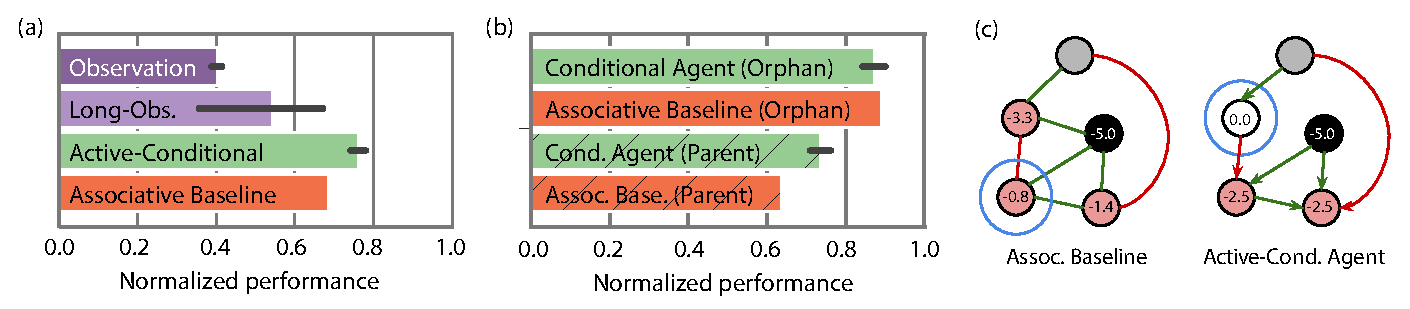
\includegraphics[width=0.99\textwidth]{figures/fig_expt1.pdf}
   %%\vspace{-0.3cm}
    \caption{\textbf{Experiment 1. Agents do causal reasoning from observational data.} a) Average performance of the agents tested in this experiment. b) Performance split by the presence or absence of at least one parent (Parent and Orphan respectively) on the externally intervened node. c) Quiz phase for a test \CBN. Green (red) edges indicate a weight of $+1$ ($-1$). Black represents the intervened node, green (red) nodes indicate a positive (negative) value, white indicates a zero value. The blue circles indicate the agent's choice. Left panel: The undirected version of ${\cal G}$ and the nodes taking the mean values prescribed by $p(X_{1:N\setminus j }|X_j=-5)$, including backward inference to the intervened node's parent. The Associative Baseline's choice is consistent with maximizing these (incorrect) node values. Right panel: ${\cal G}_{\rightarrow X_j=-5}$ and the nodes taking the mean values prescribed by $p_{\rightarrow X_j=-5}(X_{1:N\setminus j }|X_j=-5)$. The Active-Conditional Agent's choice is consistent with maximizing these (correct) node values.}%
    \label{fig:expt1}%
\end{figure}


To further demonstrate that this improvement is indeed due to causal reasoning, we partition the test cases by whether or not the node that was intervened on in the quiz phase has a parent (Figure \ref{fig:expt1}b). If the intervened node $X_j$ has no parents, then ${\cal G}  = {\cal G}_{\rightarrow X_j}$, and doing causal reasoning should afford no advantage over doing associative reasoning. Indeed, the Active-Conditional Agent performs better than the Associative Baseline only when the intervened node has parents (hatched bars in Figure \ref{fig:expt1}b). In Figure \ref{fig:expt1}c, we show the quiz phase for an example test CBN. This highlights that the Associative Baseline chooses according to the node values predicted by \(p(X_{1:N\setminus j }|X_j=-5)\), whereas the Active-Conditional Agent chooses according the node values predicted by \(p_{\rightarrow X_j=5}(X_{1:N\setminus j }|X_j=5)\)). 
%These analyses show that even given access to only observational data, the agent can learn to perform some causal reasoning.


% \begin{wrapfigure}{l}{0.27\textwidth}
% \centering
% %%\vspace{-0.4cm}
% 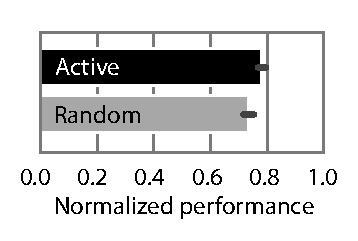
\includegraphics[width=0.3\textwidth]{figures/fig_conditional_act_v_pass.pdf}
% %%\vspace{-20pt}
% \caption{Active and Random Conditional Agents}
% % \label{fig:expt1c}
% \label{fig:expt1_active}
% %%\vspace{-0.4cm}
% \end{wrapfigure} 

%Further, we find that the Active-Conditional Agent also learns to utilize the control it has over what data it get to observe. In particular, it learns to choose informative observations and achieves significantly better performance than the Random-Conditional Agent (Figure \ref{fig:expt1_active}). This indicates that the agent is able to learns a good data collection policy when permitted.
 Comparing the performances of the Active and Random versions of the Conditional Agents, we find that the active Agent's performance is slightly but significantly ($p = 0.003$, Figure \ref{fig:expt1_extra}a) higher than the Random Agent. This indicates that when permitted, the agent learns to generate informative observations. We also trained a third agent that employs the optimal information gathering policy in the noise-free limit (acting on each visible node exactly once), and obtained a performance slightly but significantly ($p=0.008$, not shown) higher than the Active agent (although still significantly less than optimal causal reasoning), indicating that the policy learned by the Active Agent is not optimal. But the differences between the performances of agents with different information gathering policies is very small, indicating that learning a data-collection policy does not yield a critical benefit when receiving conditional samples in this small-data regime. 

Agents that receive unconditional observations from $\cal G$, i.e. the Observational Agents ("Observation" and "Long-Obs" in Figure \ref{fig:expt1}a) perform worse than the Active-Conditional Agent. Note that this is to be expected since these agents receive less diagnostic information during the information phase. However, the Observational agent is still able to leverage the information from the 4 unconditional samples it receives and perform better than the random baseline. Further, when given access to more data (the Long-Obs. agent) the same agent learns to utilize it, yielding better performance.

\begin{figure}[t!]
\centering
%%\vspace{-0.4cm}
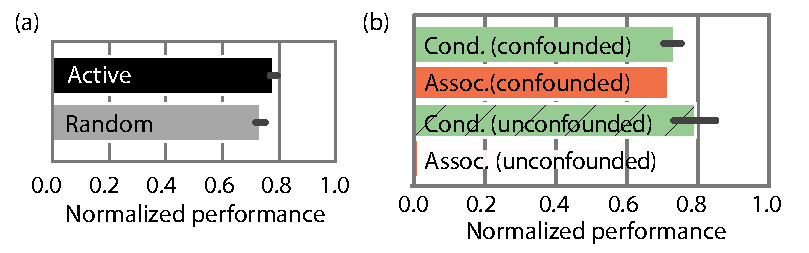
\includegraphics[width=0.8\textwidth, trim = {0 0cm 0 0.7cm}] {figures/fig2_conf_unconf_pars_act_pass_combined.pdf}
%%\vspace{-20pt}
\caption{a) Active vs Random Conditional, b)Associative Baseline vs Active Conditional, where intervened node has a parent}
% \label{fig:expt1c}
\label{fig:expt1_extra}
%%\vspace{-0.6cm}
\end{figure}

From Figure \ref{fig:expt1}a, we see that while the Active-Conditional Agent performs significantly above the Associative baseline, it far from the performance utilizing full causal reasoning (= 1.0 on our scale). From Figure \ref{fig:expt1}b, we see that this gap is driven mostly by test cases where the intervened node has a parent. While the Active-Conditional Agent's advantage over the baseline comes from these test cases, it is still not performing optimally on them. We hypothesize that this is due to the presence of unobserved confounders. As discussed in Section \ref{sec:setup}, full causal inference in the presence of confounders is in general not possible with just observational data. 
To further investigate this hypothesis, we partition the set of test cases into those where the intervened upon node has a confounded parent and those with unconfounded parents (Figure \ref{fig:expt1_extra}b). We see that the performance of the Active-Conditional Agent is significantly higher than the Associative baseline only in cases where the parent is not confounded. Causal inference in the presence of confounders is only in general possible with interventions. In the next experiment, we discuss the performance of our agents in an environment that permits interventions.

% We see however that it still cannot perform at optimal since the unobservable node might still be confounding the values of other nodes in the graph.
 
We also note that the Associative agent has higher performance when the parent of the intervened node is confounded than when it isn't (where the performance is not significantly above zero). This could point to other statistical structure in the environment -- for example, if the intervened node has more \textit{visible} parents (as is true for the graphs with unconfounded parents in Figure \ref{fig:expt1_conf}), there are more visible nodes strongly correlated with it due to (incorrect) backward inferences from child to parent. This could hinder the associative agent giving lower performance. These findings highlight that there are often unexpected statistical trends even in putatively formal settings like our distribution of simple \CBNs, that could potentially be leveraged \citep{janzing2009telling, hoyer2009nonlinear} by meta-learning agents.
% such as ours.
%  Human behavioral research also indicates that people often neglect unobserved variables \citep{fernbach2013cognitive}.
%  We leave a more detailed analyses of these statistical features to future work.

\section{Experiment 2: Interventional Environments}
\label{sec:expt2}


\begin{figure}[t!]
\centering
   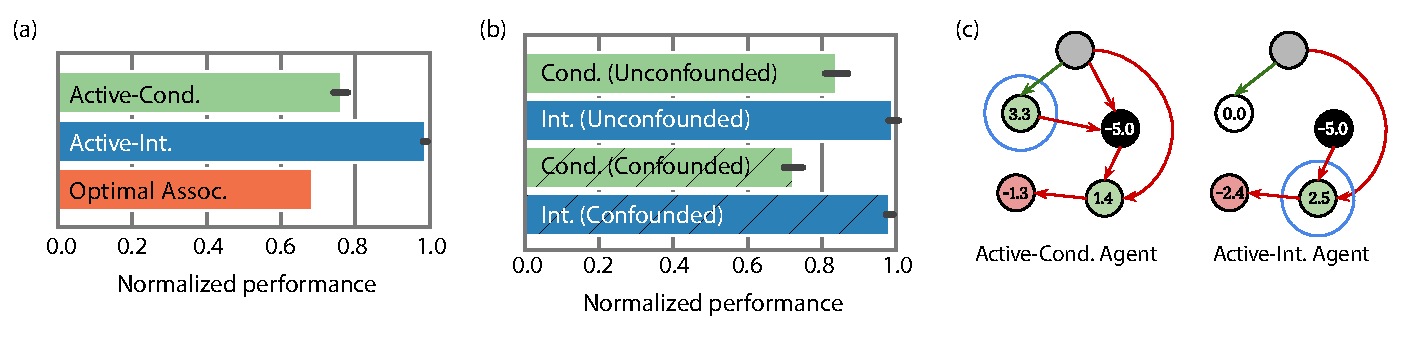
\includegraphics[width=0.99\textwidth, trim = {0 0cm 0 0.7cm}]{figures/fig_expt2.pdf}
%   %%\vspace{-0.3cm}
    \caption{\textbf{Experiment 2. Agents do causal reasoning from interventional data.} a) Average performance of the agents tested in this experiment. See main text for details. b) Performance split by the presence or absence of unobserved confounders (abbreviated as Conf. and Unconf.). c) Quiz phase for a test \CBN. See Figure \ref{fig:expt1} for a legend. Here, the left panel shows the full $\cal G$ and the nodes taking the mean values prescribed by $p(X_{1:N\setminus j }|X_j=-5)$.
    We see that the Active-Cond Agent's choice is consistent with choosing based on these (incorrect) node values. The right panel shows ${\cal G}_{\rightarrow X_j=-5}$ and the nodes taking the mean values prescribed by $p_{\rightarrow X_j=-5}(X_{1:N\setminus j }|X_j=-5)$. We see that the Active-Int. Agent's choice is consistent with maximizing on these (correct) node value.}%
    \label{fig:expt2}%
\end{figure}

In this experiment, we test if agents can learn to perform causal inference from interventions. In particular, we are interested in performance in the presence of confounders. The interventional environment allows the agent to intervene on any visible node during the information phase. The agent's actions correspond to performing an intervention on the selected node $X_j$ and sampling from ${\cal G}_{\rightarrow X_j}$ (see Section \ref{sec:task}). As discussed in Section \ref{sec:setup}, access to interventional data permits causal reasoning even in the presence of unobserved confounders, a feat in general impossible with access only to observational data. We test both active and random versions of the agent (see Section \ref{sec:task}) to disentangle if the agent can also learn to select informative interventions when the environment permits.
% \footnote{Higher performance is possible only with access to the noise re-sampled at each step. Inferring and utilizing this information is \textit{counterfactual reasoning}, see the Supplementary Material for details.}.

\subsection{Results}

The agents tested in this experiment differ from agents in previous experiments only in the kind of data that they have access to. We see in Figure \ref{fig:expt2}a that the Active-Interventional Agent's performance is better than the Active-Conditional Agent, achieving close to optimal performance. 

\begin{figure}[h]
\centering
%%\vspace{-0.4cm}
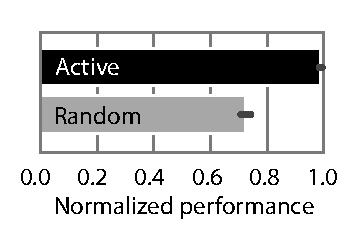
\includegraphics[width=0.3\textwidth , trim = {0 0cm 0 0.9cm}]{figures/fig_causal_act_v_pass.pdf} 
%%\vspace{-20pt}
\caption{Active and Random Interventional Agents}
\label{fig:expt2_active}
%%\vspace{-0.4cm}
\end{figure}

This shows that when given access to interventions, the agent learns to leverage them to perform causal reasoning. Partitioning the test cases by whether any node has unobserved confounders with other nodes in the graph (Figure \ref{fig:expt2}b), we see that the Active-Interventional Agent performs close to optimal on both confounded and unconfounded test cases. This confirms our hypothesis that the agent has learned to perform causal reasoning even in the presence of confounders which the Conditional agents in Experiment 1 could not do. This is highlighted by Figure \ref{fig:expt2}c, which shows the quiz phase for an example \CBN, where the Active-Conditional Agent is unable to resolve the unobserved confounder, whereas the Active-Interventional Agent is able to do so. We also see that while the performance of the Active-Conditional Agent is significantly higher in unconfounded cases than in confounded ones, it is not as high as the performance of the Interventional Agent, even though inference in the absence of confounders is in theory within reach of the conditional agent. This could be because causal inference from observations is more challenging than from interventions, in our setting. In our framework, the final quiz phase node values are the negative (with noise) of the values observed, if the quiz phase node is intervened on in the information phase\footnote{We demonstrate in Appendix \ref{app:causal_addexpt} that our agents are able to infer from interventions even in non-linear cases where the decoding is more involved.}. This makes the decoding process significantly easier than if (as with the Conditional cases), information has to be integrated across several observations in the information phase to perform well in the quiz phase. When utilizing the statistical structure of the task and environment, interventions are easy to learn from. Evidence of such behavior has also been noted in humans \citep{fernbach2013cognitive, fernbach2010neglect}.


% , even though inference in unconfounded cases should in theory be possible even with just observational data (and therefore within reach of the Conditional Agent). A possible explanation for this is that there is more information in the structure of the data extracted from interventions \citep{bengio2019meta, hoyer2009nonlinear}. In our framework, the final quiz phase node values are just the negative of the values observed if the quiz phase node is intervened on in the information phase\footnote{We demonstrate in the Supplementary Material that our agents are able to infer from interventions even in non-linear cases where the decoding is more involved.}. This makes the decoding process significantly easier than if (as with the Conditional cases), information has to be integrated across several observations in the information phase to perform well in the quiz phase. All of our experiments are in a very low data setting -- they only receive 4 samples from the \CBN, where these differences could be exacerbated. Taken together, our experiments showcase that agents can utilize statistical shortcuts that are present in the environment and the task at hand, rather than performing full formal inference. Evidence of such behavior has also been noted in humans \citep{fernbach2013cognitive, fernbach2010neglect}.

Further, we find that the Active-Interventional agent learns to utilize the control it has over what interventions it does, to choose informative interventions: its performance is significantly better than the Random-Interventional Agent (Figure \ref{fig:expt2_active}). This indicates that when permitted, the agents learns a good intervention policy to generate informative data. The difference betwee Active and Random is far greater than in the Conditional case, with the Active Interventional agent reaching ceiling performance. This indicates that in our domain, while causal inference is easier from interventions than observations, it is perhaps more sensitive to the right intervention policy -- learning a policy for information gathering yields a critical benefit above a random policy, when learning from interventions, in our domain.



\section{Experiment 3: Counterfactual Setting}
\label{sec:expt3}

In Experiment~3, the agent was again allowed to make interventions as in Experiment~2, but in this case the quiz phase task entailed answering a counterfactual question. We explain here what a counterfactual question in our experimental domain looks like. Assume $X_i = \sum_{j} w_{ji}X_{j} + \epsilon_i$ where $\epsilon_i$ is distributed as $\mathcal{N}(0.0, 0.1)$ (giving the conditional distribution $p(X_i \vert \textrm{pa}(X_{i})) = \mathcal{N}(\sum_{j} w_{ji}X_{j},0.1)$ as described in Section 3). After observing the nodes $X_{2:N}$ ($X_{1}$ is hidden) in the \CBN~in one sample, we can infer this latent randomness $\epsilon_i$ for each observable node $X_i$ (i.e.~\textit{abduction}) and answer counterfactual questions like "What would the values of the nodes be, had $X_i$ instead taken on a different value than what we observed?", for any of the observable nodes $X_i$. We test three new agents, two of which are learned: "Active Counterfactual", "Random Counterfactual", and "Optimal Counterfactual Baseline" (not learned).


\paragraph{Counterfactual Agents:}
This agent is the same as the Interventional agent, but trained on tasks in which the latent randomness in the last information phase step $t = T-1$ (where some $X_p=+5$) is stored and the same randomness is used in the quiz phase step $t = T$ (where some $X_f=-5$). While the question our agents have had to answer correctly so far in order to maximize their reward in the quiz phase was "Which of the nodes $X_{2:N}$ will have the highest value when $X_f$ is set to $-5$?", in this setting, we ask "Which of the nodes $X_{2:N}$ would have had the highest value in the last step of the information phase, if instead of having the intervention $X_p=+5$,  we had the intervention $X_f = -5$?".
We run active and random versions of this agent as described in the main text.

\paragraph{Optimal Counterfactual Baseline:}
This baseline receives the true \CBN~and does exact abduction of the latent randomness based on observations from the penultimate step of the information phase, and combines this correctly with the appropriate interventional inference on the true \CBN~in the quiz phase.


\begin{figure}[t!]
\centering
   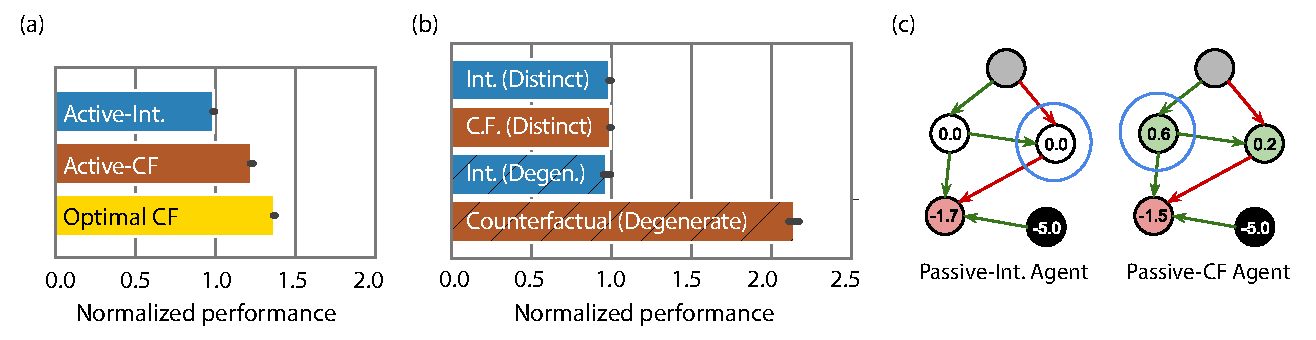
\includegraphics[width=0.95\textwidth]{figures/fig_expt3.pdf}
%   %\vspace{-0.3cm}
    \caption{Experiment 3.  Agents do counterfactual reasoning. a) Performance of the agents tested in this experiment. Note that performance can be above 1.0 since the counterfactual agent can theoretically perform better than the optimal interventional baseline, which doesn't have access to noise information. See main text for details. b) Performance split by if the maximum node value in the quiz phase is degenerate (Deg.) or distinct (Dist.). c) Quiz phase for an example test-CBN. See Figures in Main text for a legend. Here, the left panel shows ${\cal G}_{\rightarrow X_j=-5}$ and the nodes taking the mean values prescribed by $p_{\rightarrow X_j=-5}(X_{1:N\setminus j }|X_j=-5)$. We see that the Active-Int. Agent's choice is consistent with maximizing on these node values, where it makes a random choice between two nodes with the same value. The right panel panel shows ${\cal G}_{\rightarrow X_j=-5}$ and the nodes taking the exact values prescribed by the means of $p_{\rightarrow X_j=-5}(X_{1:N\setminus j }|X_j=-5)$, combined with the specific randomness inferred from the previous time step. As a result of accounting for the randomness, the two previously degenerate maximum values are now distinct. We see that the Active-CF. agent's choice is consistent with maximizing on these node values.}%
    \label{fig:expt3}%
\end{figure}



\subsection{Results}

We focus on two key questions in this experiment. 
(i) Do our agents learn to do counterfactual inference? The Active-Counterfactual Agent achieves higher performance than the maximum possible performance using only causal reasoning (Figure \ref{fig:expt3}a). This indicates that the agent learns to infer and apply noise information from the last step of the information phase. To evaluate whether this difference is driven by the agent's use of abduction, we split the test set into two groups, depending on whether or not the decision for which node will have the highest value in the quiz phase is affected by the latent randomness, i.e. whether or not the node with the maximum value in the quiz phase changes if the noise is resampled.
This is most prevalent in cases where the maximum expected reward is degenerate, i.e. where several nodes give the same maximum reward (denoted by hatched bars in Figure \ref{fig:expt3}b). Here, agents with no access to the randomness have no basis for choosing one over the other, but different noise samples can give rise to significant differences in the actual values that these degenerate nodes have. 

\begin{figure}[h]
\centering
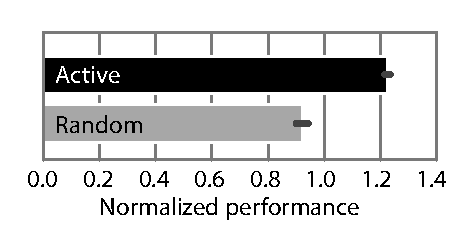
\includegraphics[width=0.3\textwidth]{figures/fig_counterfactual_act_v_pass.pdf} 
\caption{Active and Random Counterfactual Agents}
\label{fig:expt3_active}
\end{figure}

We see indeed that there is no difference in the rewards received by the Active-Counterfactual and Active-Interventional Agents in the cases where the maximum values are distinct, however the Active-Counterfactual Agent significantly outperforms the Active-Interventional Agent in cases where there are degenerate maximum values. This performance increase is very high since in most cases where the maximum values are degenerate, this maximum value is close to 0.0. Thus, taking the noise into account gives the Counterfactual agent a huge relative advantage in these cases.

(ii) Do our agents learn to make useful interventions in the service of a counterfactual task?  The Active-Counterfactual Agent's performance is significantly greater than the Random-Counterfactual Agent's (Figure \ref{fig:expt3_active}). This indicates that when the agent is allowed to choose its actions, it makes tailored, non-random choices about the interventions it makes and the data it wants to observe -- even in the service of a counterfactual objective. 



\section{Discussion and Future Work}

Learning abstract structural information about the world that generalizes across tasks is an important component of natural intelligence underlying its flexibility and data-efficiency. In this chapter, I show that causal reasoning capabilities can arise from such hierarchical structure learning (i.e. meta-learning) simply through interaction with an environment that rewards and permits causal reasoning. An important prediction of our model is that different kinds and extents of causal reasoning can arise depending on existing structure in the environment. We find that when put in different environments, our agents learn to: 1) leverage observational data to make causal inferences, 2) leverage interventions to perform causal inference in the presence of unobserved confounders, 3) leverage instance-specific information to perform counterfactual reasoning, and 4) perform active-learning, i.e. actively generate informative data when the environment permits it. 

Even in this simple domain, we saw evidence of unspecified, non-trivial underlying statistical structure in the environment, as well as preliminary evidence that our agents utilize it via heuristics. Future work could further examine the procedures being learned and the kinds of structure being utilized. In our analyses, we compared to baselines and study behavior on diagnostic test-sets to characterize these. Other work on statistical approaches to learning causal structure \citep{bengio2019meta, janzing2009telling, hoyer2009nonlinear}, as well as methods from neuroscience \citep{wang2018}, could provide further insights into what our agents learn, which could potentially be leveraged for more efficient causal reasoning. By using an RL framework, our agents learn to take actions that produce useful information---opening up possibilities for structured exploration, and optimal experiment design. In our work, we don't address the causal grounding problem---our agents are told what the relevant variables are. Using models that are more explicitly structured \citep[e.g.][]{andreas2016neural,battaglia2018relational, ganin2018synthesizing}, and more advanced architectures \citep[e.g.][]{hester2017deep,hessel2018multi,espeholt2018impala}, could allow us to scale up to directly inferring more systematic representations from unstructured input, and perform a larger range of tasks. The unique advantages of our model-free, discriminative approach is that it learns causal induction (inferring the causal structure, i.e. acquiring ``potential knowledge'' of the domain) and causal inference (making predictions about causal events, i.e. converting potential knowledge to ``realized knowledge'') end to end. Therefore the causal structure implicitly represented is influenced by the downstream inferences. This is ecologically rational and could allow us to isolate relevant causal variables in a domain, to then feed into a more structured approach to causal induction, thereby reducing the computational costs of this search.

% The results here are a first step in these directions,  would allow us to scale up our approach. 



% interesting directions for research in machine learning. Meta-learning can 
% % leverage the flexibility of deep-learning to 
% represent structure in the problem domain that may be too complex to know a priori and specify in formal models \citep{duan2016RL2,santoro2016meta,wang2016}, allowing more efficient and accurate causal reasoning. By using an RL framework, our agents can learn to take actions that produce useful information---i.e. perform active learning. This opens up possibilities for agents that perform experiments to support structured exploration in RL, and learning optimal experiment design in complex domains where interventions, or extensive data collection, are prohibitive. The results here are a first step in these directions as they obtained using relatively standard deep RL components. More advanced architectures \citep[e.g.][]{hester2017deep,hessel2018multi,espeholt2018impala} would allow us to scale up our approach to larger environments with more complex causal structure and a more diverse range of tasks. In our current work, we don't address the crucial issue of reasoning from pixels, our agents receive very structured input and don't need to infer what the relevant variables are (i.e. the causal grounding problem). Further, their representation of these variables is not systematic or compositional. Using models that are more explicitly structured \citep[e.g.][]{andreas2016neural,battaglia2018relational, ganin2018synthesizing} can allow us to scale up to directly inferring more systematic representations from unstructured input, thus potentially providing us with better sample efficiency (in the outer loop of training) and better generalization.

A crucial contribution of our work is to consider causal reasoning in natural intelligence not an end in and of itself but a means to better performance on some downstream task that is easier to specify, in a world that contains causal structure. In our case this task is acquiring reward in an RL task, but could be generalized to any other task by simply changing the meta-learning objective. This is a reasonable assumption since causal reasoning exists in humans, and even chimpanzees and rats \citep{blaisdell2006causal,gopnik2004theory,premack1994levels} without ``formal instruction'' on causality itself. This assumption allows us to frame the acquisition of causal reasoning as a meta-learning problem, and we highlight how this approach could also capture many qualitative empirical findings in how causal reasoning is learned and implemented in humans.

This direction of research opens up many interesting directions in cognitive science and psychology. We focused primarily on varying the kinds of data available to the agent, but there many other ways in which the agent's experience will inform the kind and extent of causal reasoning exhibited. In this study, we uniformly sample the space of \CBNs~and external interventions, but ecological distributions of causal structures and queries are not uniformly distributed and vary significantly from domain to domain. Our meta-learning framework adapts to such structure in the training distribution \citep{duan2016RL2,ortega2019meta,wang2016} and could parallel the domain/function specificity of human causal reasoning \citep{krynski2007role, lombrozo2010causal}. Different distributions of queries can also create situations where simpler associative strategies are largely indistinguishable from full causal reasoning \citep{todd2007environments, gigerenzer2009homo}. For example, as in Experiment 1, when the intervened upon node has no parents, causal reasoning is equivalent to associative reasoning. Further, in most real-world tasks, causal inference is usually not useful in and of itself, but rather for some downstream task. The reward in our study also depended only indirectly on causal reasoning. While in our task, causal reasoning is still an optimal strategy, this may not always be the case. These factors may result in different optimal strategies that vary on the spectrum of how ``causally-aware'' they are, and allow parallels to the graded notions of causal inference in humans \citep{fernbach2010neglect, fernbach2013cognitive, rehder2014independence, rehder2017failures}. 
% Another interesting direction is whether the developmental trajectory of our meta-learning agent matches that observed in human infants and children, i.e. what are the kinds of reasoning that .

% One drawback of our current approach is that it does not scale well with the number of nodes. However, much evidence in both the natural and artificial intelligence  This concern is intimately linked with another crucial issue of frame and representation. While  -- our agents are already given what the relevant variables are.  and more expressive models

% \jane{weaknesses: 1. we don't address the representation problem, we simply give the agent the correct representation (ie it doesn't need to infer what are the salient variables), but this is perhaps an orthogonal, although very crucial, issue. 2. Meta-RL doesn't scale well with the NUMBER of nodes. But neither do humans, who often can't keep more than a few causal factors in mind at any given time (c.f. Bengio's consciousness prior \citep{bengio2017consciousness}). (To do that, we need to build in more inductive biases via eg graph nets, which does lead to better data efficiency, although this data is not shown).}
